\documentclass[12pt]{article}

\usepackage[margin=1in, left=0.6in, right=0.6in]{geometry}
\usepackage{fancyhdr} % header
\usepackage{hyperref} % links
\usepackage{amsmath,amsthm,amssymb} %math stuff
\usepackage{setspace} % increase line spacing
\usepackage[table]{xcolor} % align environment
% \usepackage{color, soul}
\usepackage{changepage} % for the adjustwidth environment
\usepackage{relsize} % Scaling the font
\usepackage{graphicx} \graphicspath{ {./images/} } % images
\usepackage{tabularx} % long tables
\usepackage{makecell} % newlines in a table cell
\usepackage{xfrac} % slanted fractions

\definecolor{gray}{rgb}{0.5,0.5,0.5}

\setlength{\parindent}{0pt}
\everymath{\displaystyle}

\pagestyle{fancy}
\fancyhead[LO,L]{CSCD58 Assignment 1}
\fancyhead[CO,C]{Stephen Guo}
\fancyhead[RO,R]{1006313231}
\fancyfoot[LO,L]{}
\fancyfoot[CO,C]{\thepage}
\fancyfoot[RO,R]{}

\begin{document}
%----------------------------------------------------------------------------------
%                              Table of Contents
%----------------------------------------------------------------------------------
\begin{center}
	\hypertarget{toc}{\LARGE \underline{\textbf{Table of Contents}}}\\
\end{center}

{\textbf{Question 1:}}
\vspace{1mm}
\hrule
\vspace{1mm}
\hyperlink{1.1}{(a)}\\
\hyperlink{1.2}{(b)}\\
\\

{\textbf{Question 2:}}
\vspace{1mm}
\hrule
\vspace{1mm}
\hyperlink{2.1}{(a)}\\
\hyperlink{2.2}{(b)}\\
\hyperlink{2.3}{(c)}\\
\hyperlink{2.4}{(d)}\\
\hyperlink{2.5}{(e)}\\
\hyperlink{2.6}{(f)}\\
\hyperlink{2.7}{(g)}\\
\\

{\textbf{Question 3:}}
\vspace{1mm}
\hrule
\vspace{1mm}
\hyperlink{3.1}{(a)}\\
\hyperlink{3.2}{(b)}\\
\hyperlink{3.3}{(c)}\\
\hyperlink{3.4}{(d)}\\
\\

{\textbf{Question 4:}}
\vspace{1mm}
\hrule
\vspace{1mm}
\hyperlink{4.1}{(a)}\\
\hyperlink{4.2}{(b)}\\
\hyperlink{4.3}{(c)}\\
\hyperlink{4.4}{(d)}\\
\\

\hyperlink{5}{\textbf{Question 5:}}
\vspace{1mm}
\hrule
~\\

{\textbf{Question 6:}}
\vspace{1mm}
\hrule
\vspace{1mm}
\hyperlink{6.1}{(a)}\\
\hyperlink{6.2}{(b)}\\
\hyperlink{6.3}{(c)}\\
\\

{\textbf{Question 7:}}
\vspace{1mm}
\hrule
\vspace{1mm}
\hyperlink{7.1}{(a)}\\
\hyperlink{7.2}{(b)}\\
\hyperlink{7.3}{(c)}\\
\\

{\textbf{Question 8:}}
\vspace{1mm}
\hrule
\vspace{1mm}
\hyperlink{8.1}{(a)}\\
\hyperlink{8.2}{(b)}\\
\\

\newpage

%----------------------------------------------------------------------------------
%                                   Questions
%----------------------------------------------------------------------------------
\setstretch{1.2}
%----------------------------------------------------------------------------------
% !                                     1
%----------------------------------------------------------------------------------
\hyperlink{toc}{\LARGE \underline{\textbf{Question 1.}}}\\
~\\\hyperlink{toc}{\hypertarget{1.1}{(a)}}\\
$\frac{L}{R} \times N$\\
~\\\hyperlink{toc}{\hypertarget{1.2}{(b)}}\\
$P \times \frac{L}{R} + \frac{L}{R} \times (N-1)$\\
$P \times \frac{L}{R}$ for transmitting all packets, and $\frac{L}{R} \times (N-1)$ to transmit the last packet through all switches.
\newpage

%----------------------------------------------------------------------------------
% !                                     2
%----------------------------------------------------------------------------------
\hyperlink{toc}{\LARGE \underline{\textbf{Question 2.}}}\\
~\\\hyperlink{toc}{\hypertarget{2.1}{(a)}}\\
$d_{\text{prop}} = \frac{m}{s}$\\
~\\\hyperlink{toc}{\hypertarget{2.2}{(b)}}\\
$d_{\text{trans}} = \frac{L}{R}$\\
~\\\hyperlink{toc}{\hypertarget{2.3}{(c)}}\\
$d_{\text{end-to-end}} = \frac{m}{s} + \frac{L}{R}$\\
~\\\hyperlink{toc}{\hypertarget{2.4}{(d)}}\\
Right after starting of the host link\\
~\\\hyperlink{toc}{\hypertarget{2.5}{(e)}}\\
% S times propogation speed
Still in the link. $d_{\text{trans}} \times s$ meters into the link. % $\frac{m}{s} + \frac{L}{R}$ into the link\\
~\\\hyperlink{toc}{\hypertarget{2.6}{(f)}}\\
In the host B\\
~\\\hyperlink{toc}{\hypertarget{2.7}{(g)}}\\
$d_{\text{prop}} = \frac{m}{s} = \frac{m}{2.5\times 10^{8}\ m/s}$\\
$d_{\text{trans}} = \frac{120\ \text{bits}}{56\ 000\ \text{bits/s}} = \frac{3\ \text{bits}}{1\ 400\ \text{bits/s}}$\\

Then if $d_{\text{prop}} = d_{\text{trans}}$, we have\\
$$
	\begin{array}{r@{}>{\displaystyle}l}
		\frac{m}{2.5\times 10^{5}\ m/s} & {} =  \frac{3\ \text{bits}}{1\ 400\ \text{bits/s}}                         \\
		m \times 1400\ \text{bits/s}    & {} =3\ \text{bits}\times 2.5 \times 10^8\ m/s                              \\
		m                               & {} = \frac{3\ \text{bits}\times 2.5 \times 10^8\ m/s}{1400\ \text{bits/s}} \\
		m                               & {} \approx     535\ 714.2857\ m                                            \\
	\end{array}
$$
\newpage

%----------------------------------------------------------------------------------
% !                                     3
%----------------------------------------------------------------------------------
\hyperlink{toc}{\LARGE \underline{\textbf{Question 3.}}}\\
~\\\hyperlink{toc}{\hypertarget{3.1}{(a)}}\\
$\frac{3 \times 10^6\ \text{bits/s}}{150 \times 10^3\ \text{bits/s}} = 20$\\

~\\\hyperlink{toc}{\hypertarget{3.2}{(b)}}\\
10\%\\

~\\\hyperlink{toc}{\hypertarget{3.3}{(c)}}\\
Binomial Distribution: $P = \binom{n}{x}p^x (1-p)^{n-x}$\\
$$
	\begin{array}{r@{}>{\displaystyle}l}
		x & {} = n            \\
		n & {} = 120          \\
		p & {} = \frac{1}{10} \\
	\end{array}
$$
So $P(X=n) = \binom{120}{n}\left(0.1\right)^n \left(0.9\right)^{120-n}$

~\\\hyperlink{toc}{\hypertarget{3.4}{(d)}}\\
Binomial Distribution: $P = \binom{n}{x}p^x (q-p)^{n-x}$\\

Want probability of $x=21,\ x=22,\ \cdots\ ,\ x=119,\ x=120$\\
$$
	\begin{array}{r@{}>{\displaystyle}l}
		P(X \geq 21) & {} = \sum_{n=21}^{120} \binom{120}{n}0.1^n (0.9)^{120-n} \\
		             & {} \approx 0.00794                                       \\
	\end{array}
$$
\newpage

%----------------------------------------------------------------------------------
% !                                     4
%----------------------------------------------------------------------------------
\hyperlink{toc}{\LARGE \underline{\textbf{Question 4.}}}\\
~\\\hyperlink{toc}{\hypertarget{4.1}{(a)}}\\
% \textbf{Note}: Assuming the
% $\frac{1.5 \times 10^6\ \text{bytes}}{1 \times 10^3\ \text{bytes}} = 1\ 500\ \text{packets}$\\
% \\
$$
	\begin{array}{r@{}>{\displaystyle}l}
		\text{Transfer Time} & {} = \frac{\text{Transfer Size}}{\text{Bandwidth}}                                 \\[6mm]
		                     & {} = \frac{1.5 \times 2^{20} \text{ bits }}{10 \times 10^{6} \text{ bits/second }} \\[6mm]
		                     & {} = 1.2582912 \text{ seconds }                                                    \\[6mm]
	\end{array}
$$\\

$$
	\begin{array}{r@{}>{\displaystyle}l}
		\text{Total time} & {} = \text{Handshake + Transfer Time}                                          \\
		                  & {} = (2\times 80 \times 10^{-3} \text{ seconds)} + (1.2582912 \text{ seconds}) \\
		                  & {} = 1.4182912 \text{ seconds}                                                 \\
	\end{array}
$$\\

~\\\hyperlink{toc}{\hypertarget{4.2}{(b)}}\\
$\frac{1.5 \times 2^{20}\ \text{bytes}}{1 \times 2^{10}\ \text{bytes}} = 1\ 536\ \text{packets}$\\
$$
	\begin{array}{r@{}>{\displaystyle}l}
		\text{Time for one packet} & {} = \text{Transfer Time}                                                                 \\
		                           & {} = \frac{1 \times 2^{10} \times 8 \text{ bits }}{10 \times 10^{6} \text{ bits/second }} \\
		                           & {} = 0.0008192 \text{ seconds}                                                            \\
	\end{array}
$$\\

$$
	\begin{array}{r@{}>{\displaystyle}l}
		\text{Total time} & {} = \text{Handshake} + 1\ 536 \times \text{Time for one packet} + 1\ 535 \text{ RTT}                                                                      \\
		                  & {} = (2\times 80 \times 10^{-3} \text{ seconds}) + 1\ 536 \times 0.0008192 \text{ seconds } + 1\ 535 \times \left(80 \times 10^{-3} \text{ seconds}\right) \\
		                  & {} = 124.2182912 \text{ seconds}                                                                                                                           \\
	\end{array}
$$\\


~\\\hyperlink{toc}{\hypertarget{4.3}{(c)}}\\
$\frac{1.5 \times 2^{20}\ \text{bytes}}{1 \times 2^{10}\ \text{bytes}} = 1\ 536\ \text{packets}$\\

$\frac{1\ 536\text{ packets}}{20 \text{ packets/RTT}} = 76.8 \text{ RTT} = 76 \text{ RTT}$\\

$76 \text{ RTT} \times 80 \times 10^{-3} \text{ seconds/RTT} = 6.08 \text{ seconds}$\\
$$
	\begin{array}{r@{}>{\displaystyle}l}
		\text{Total time} & {} = \text{Handshake} + \left(76 \text{ RTT} \times 80 \times 10^{-3} \text{ seconds/RTT}\right) \\
		                  & {} = \left(2\times 80 \times 10^{-3} \text{ seconds}\right) + 6.08 \text{ seconds}               \\
		                  & {} = 6.24 \text{ seconds}                                                                        \\
	\end{array}
$$\\

~\\\hyperlink{toc}{\hypertarget{4.4}{(d)}}\\
$\frac{1.5 \times 2^{20}\ \text{bytes}}{1 \times 2^{10}\ \text{bytes}} = 1\ 536\ \text{packets}$\\

Sum of powers of 2 is the biggest binary number = $2^n-1$\\
% Sum of squares series = $\frac{n(n+1)(2n+1)}{6}$\\

for $n = 10$, the sum of powers of 2 is 1023.\\
for $n = 11$, the sum of powers of 2 is 2047.\\
Therefore, there is going to be 10 RTT.\\

$$
	\begin{array}{r@{}>{\displaystyle}l}
		\text{Total time} & {} = \text{Handshake} + 10 \text{ RTT} \times 80 \times 10^{-3} \text{ seconds/RTT} \\
		                  & {} = \left(2\times 80 \times 10^{-3} \text{ seconds}\right) + 0.8 \text{ seconds}   \\
		                  & {} = 0.96 \text{ seconds}                                                           \\
	\end{array}
$$
% $11 \text{ RTT} \times 80 \times 10^{-3} \text{ seconds/RTT} = 0.88 \text{ seconds}$\\
\newpage

%----------------------------------------------------------------------------------
% !                                     5
%----------------------------------------------------------------------------------
\hyperlink{toc}{\hypertarget{5}{\LARGE \underline{\textbf{Question 5.}}}}\\
Propogation Delay = $\frac{\text{Distance}}{\text{Propogation Speed}}$\\[6mm]
Transmission Delay = $\frac{\text{Size}}{\text{Bandwidth}}$\\

Setting them equal for 100-byte packets, we have
$$
	\begin{array}{r@{}>{\displaystyle}l}
		\frac{\text{Distance}}{\text{Propogation Speed}}             & {} = \frac{\text{Size}}{\text{Bandwidth}}                                          \\[6mm]
		\frac{50 \times 10^{3} \text{ m }}{2\times10^8 \text{ m/s }} & {} = \frac{100 \times 8 \text{ bits }}{\text{Bandwidth}}                           \\[6mm]
		\text{Bandwidth} \times \left(50\ 000 \text{ m}\right)       & {} = (2 \times 10^8 \text{ m/s})\times(800 \text{ bits})                           \\[6mm]
		\text{Bandwidth}                                             & {} = \frac{(2 \times 10^8 \text{ m/s})\times(800 \text{ bits})}{50\ 000 \text{ m}} \\[6mm]
		                                                             & {} =   3\ 200\ 000 \text{ bits/s}                                                  \\[6mm]
	\end{array}
$$\\

Setting them equal for 512-byte packets, we have
$$
	\begin{array}{r@{}>{\displaystyle}l}
		\text{Bandwidth} & {} = \frac{(2 \times 10^8 \text{ m/s})\times(512 \times 8 \text{ bits})}{50\ 000 \text{ m}} \\[6mm]
		                 & {} =   16\ 384\ 000 \text{ bits/s}                                                          \\[6mm]
	\end{array}
$$
\newpage

%----------------------------------------------------------------------------------
% !                                     6
%----------------------------------------------------------------------------------
\hyperlink{toc}{\LARGE \underline{\textbf{Question 6.}}}\\
~\\\hyperlink{toc}{\hypertarget{6.1}{(a)}}\\
For the shortest RTT, we would want to transmit only 1 bit, so we can ignore transmit delay.\\
$$
	\begin{array}{r@{}>{\displaystyle}l}
		\text{RTT} & {} = 2 \times \text{Propagation}                                                     \\[6mm]
		           & {} = 2 \times \frac{\text{Distance}}{\text{Propagation speed}}                       \\[6mm]
		           & {} = 2\times \frac{55 \times 10^9 \text{ meters}}{3\times10^8 \text{ meters/second}} \\[6mm]
		           & {} = 366 + \frac{2}{3} \text{ seconds}                                               \\[6mm]
		% & {} =                                                                                \\[6mm]
	\end{array}
$$

~\\\hyperlink{toc}{\hypertarget{6.2}{(b)}}\\
$$
	\begin{array}{r@{}>{\displaystyle}l}
		\text{delay} \times \text{bandwidth} & {} = 366 + \frac{2}{3} \text{ seconds} \times 128 \times 10^3 \text{ bits/second} \\[6mm]
		                                     & {} = 46\ 933\ 333 + \frac{1}{3} \text{ bits}                                      \\[6mm]
		                                     & {} = 46\ 933\ 333 \text{ bits}                                                    \\[6mm]
	\end{array}
$$
% delay $\times$ bandwidth = $366 + \frac{2}{3} \text{ seconds} \times 128 \times 10^3 \text{ bits/second}$
% $= 46933333 + \frac{1}{3}$
~\\\hyperlink{toc}{\hypertarget{6.3}{(c)}}\\
$$
	\begin{array}{r@{}>{\displaystyle}l}
		% DO half of RTT!!!
		\text{Transfer time} & {} = \frac{\text{RTT}}{2} + \frac{\text{Transfer size}}{\text{Bandwidth}}                                                                          \\[6mm]
		                     & {} = \frac{1}{2}\left(366 + \frac{2}{3}\right) \text{ seconds} + \frac{5 \times 8 \times 2^{20} \text{ bits}}{128 \times 10^3 \text{ bits/second}} \\[6mm]
		                     & {} = 511 + \frac{1}{75} \text{ seconds}                                                                                                            \\[6mm]
		                     & {} = 511.01\overline{3} \text{ seconds}                                                                                                            \\[6mm]
	\end{array}
$$
% $$
% 	\begin{array}{r@{}>{\displaystyle}l}
% 		 & {} =  \\
% 		 & {} =  \\
% 		 & {} =  \\
% 	\end{array}
% $$
\newpage

%----------------------------------------------------------------------------------
% !                                     7
%----------------------------------------------------------------------------------
\hyperlink{toc}{\LARGE \underline{\textbf{Question 7.}}}\\
~\\\hyperlink{toc}{\hypertarget{7.1}{(a)}}\\
% % this is if there's 1 extra processing
% $$
% 	\begin{array}{r@{}>{\displaystyle}l}
% 		\text{Transmit time} & {} = \frac{\text{Size}}{\text{Bandwidth}}                          \\[6mm]
% 		                     & {} = \frac{5\ 000 \text{ bits}}{1 \times 10^9 \text{ bits/second}} \\[6mm]
% 		                     & {} = \frac{1}{200000} \text{ seconds}                              \\[6mm]
% 		                     & {} = 5 \times 10^{-6} \text{ seconds}                              \\[6mm]
% 		                     & {} = 0.000005 \text{ seconds}                                      \\[6mm]
% 	\end{array}
% $$
%
% Since there is 1 router, there is 2 links to pass through.
% $$
% 	\begin{array}{r@{}>{\displaystyle}l}
% 		\text{Transfer Time} & {} = 2 \times \text{Propogation} + 3 \times \text{Transmit}                                                          \\
% 		                     & {} = 2 \times \left(10 \times 10^{-6} \text{ seconds}\right) + 3\times \left(5 \times 10^{-6} \text{ seconds}\right) \\
% 		                     & {} = 3.5 \times 10^{-5} \text{ seconds}                                                                              \\
% 		                     & {} = 0.000035 \text{ seconds}                                                                                        \\
% 	\end{array}
% $$
%
% ~\\\hyperlink{toc}{\hypertarget{7.2}{(b)}}\\
% For 3 switches, there will be 4 links.
% $$
% 	\begin{array}{r@{}>{\displaystyle}l}
% 		\text{Transfer Time} & {} = 4 \times \text{Propogation} + 5 \times {Transmit}                                                       \\
% 		                     & {} = 4 \times \left(10 \times 10^{-6} \text{ seconds}\right) + 5 \times \left(10^{-6} \text{ seconds}\right) \\
% 		                     & {} = 6.5 \times 10^{-5} \text{ seconds}                                                                      \\
% 		                     & {} = 0.000065 \text{ seconds}                                                                                \\
% 	\end{array}
% $$
$$
	\begin{array}{r@{}>{\displaystyle}l}
		\text{Transmit time} & {} = \frac{\text{Size}}{\text{Bandwidth}}                          \\[6mm]
		                     & {} = \frac{5\ 000 \text{ bits}}{1 \times 10^9 \text{ bits/second}} \\[6mm]
		                     & {} = \frac{1}{200000} \text{ seconds}                              \\[6mm]
		                     & {} = 5 \times 10^{-6} \text{ seconds}                              \\[6mm]
		                     & {} = 0.000005 \text{ seconds}                                      \\[6mm]
	\end{array}
$$

Since there is 1 router, there is 2 links to pass through.
$$
	\begin{array}{r@{}>{\displaystyle}l}
		\text{Transfer Time} & {} = 2 \times \text{Propogation} + 3 \times \text{Transmit}                                      \\
		                     & {} = 2 \times \left(10 \times 10^{-6} \text{ seconds } + 5 \times 10^{-6} \text{ seconds}\right) \\
		                     & {} = 3 \times 10^{-5} \text{ seconds}                                                            \\
		                     & {} = 0.00003 \text{ seconds}                                                                     \\
	\end{array}
$$

~\\\hyperlink{toc}{\hypertarget{7.2}{(b)}}\\
For 3 switches, there will be 4 links.
$$
	\begin{array}{r@{}>{\displaystyle}l}
		\text{Transfer Time} & {} = 4 \times \text{Propogation + Transmit}                                                                  \\
		                     & {} = 4 \times \left(10 \times 10^{-6} \text{ seconds}\right) + 5 \times \left(10^{-6} \text{ seconds}\right) \\
		                     & {} = 6 \times 10^{-5} \text{ seconds}                                                                        \\
		                     & {} = 0.00006 \text{ seconds}                                                                                 \\
	\end{array}
$$
~\\\hyperlink{toc}{\hypertarget{7.3}{(c)}}\\
$$
\text{Transmit time}_{5\ 000} = 5 \times 10^{-6} \text{ seconds}                                \\[6mm]
$$

	If a switch can retransmit after 128 bits, it will only be effective for the last 2 switches. so we have:
$$
\begin{array}{r@{}>{\displaystyle}l}
	\text{Transmit time}_{128} & {} = \frac{\text{Size}}{\text{Bandwidth}}                       \\[6mm]
	                           & {} = \frac{128 \text{ bits}}{1 \times 10^9 \text{ bits/second}} \\[6mm]
	                           & {} = \frac{1}{7812500} \text{ seconds}                          \\[6mm]
	                           & {} = 1.28 \times 10^{-7} \text{ seconds}                        \\[6mm]
	                           & {} = 0.000000128 \text{ seconds}                                \\[6mm]
\end{array}
$$

$$
\begin{array}{r@{}>{\displaystyle}l}
	\text{Transfer Time} & {} = 4 \times \text{Propogation} + 3 \times \text{Transmit time}_{128} + \text{Transmit time}_{5\ 000}                                                        \\
	                     & {} =  4 \times \left(10 \times 10^{-6} \text{ seconds} \right) + 3 \times \left(1.28 \times 10^{-7} \text{ seconds}\right) + 5 \times 10^{-6} \text{ seconds} \\
	                     & {} =\frac{5673}{125000000}\text{ seconds}                                                                                                                     \\
	                     & {} = 0.000045384 \text{ seconds}                                                                                                                              \\
	                     & {} = 4.5384 \times 10^{-5} \text{ seconds}                                                                                                                    \\
\end{array}
$$
	\newpage

	%----------------------------------------------------------------------------------
	% !                                     8
	%----------------------------------------------------------------------------------
	\hyperlink{toc}{\LARGE \underline{\textbf{Question 8.}}}\\
	~\\\hyperlink{toc}{\hypertarget{8.1}{(a)}}\\
$$
\begin{array}{r@{}>{\displaystyle}l}
	\text{Total Delay} & {} = \text{Queuing delay + Transmission delay} \\[6mm]
	                   & {} = \frac{IL}{R(1-I)} + \frac{L}{R}           \\[6mm]
\end{array}
$$

	~\\\hyperlink{toc}{\hypertarget{8.2}{(b)}}\\
	Substituting $x=\frac{L}{R}$, we have:
$$
\begin{array}{r@{}>{\displaystyle}l}
	\text{Total delay} & {} = \frac{IL}{R(1-I)} + \frac{L}{R}          \\[6mm]
	                   & {} = \frac{x^2a}{1-xa} + x                    \\[6mm]
	                   & {} = \frac{x^2a}{1-xa} + \frac{x(1-xa)}{1-xa} \\[6mm]
	                   & {} = \frac{x^2a + x(1-xa)}{1-xa}              \\[6mm]
	                   & {} = \frac{x^2a + x - x^2a}{1-xa}             \\[6mm]
	                   & {} = \frac{x}{1-xa}                           \\[6mm]
\end{array}
$$
\begin{center}
	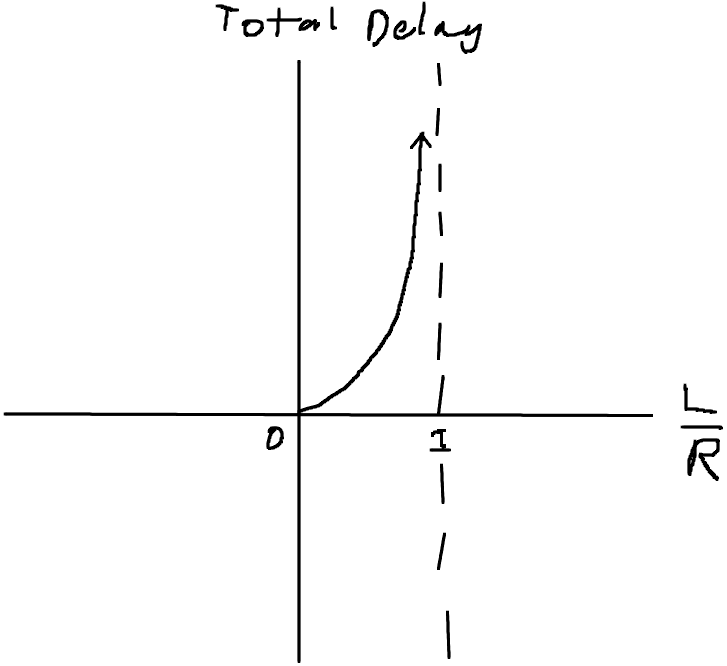
\includegraphics[width=10cm]{cscd58-a1-q8-b.png}
\end{center}
\end{document}

